\section{Modeling}

\subsection{Select Modeling Technique}

The modeling task is binary classification for \texttt{review\_concern}. A positive example is a pull request that later receives a substantive concern signal during review; a negative example has review activity but no such signal. The task is difficult because the model only sees information available at pull request opening time, while the label is determined by later reviewer behavior.

Five model candidates were compared. The majority-class baseline measures how much can be achieved by exploiting class imbalance only. Logistic regression is used as a linear reference, first on tabular pull request features and then on the full feature set. XGBoost is used as the main non-linear candidate because it can combine numeric metadata, sparse indicators, and dense diff embeddings. The all-feature models use 802 features, including the 768-dimensional capped ModernBERT representation of the source-code diff.

\subsection{Generate Test Design}

The repository-level split from data preparation is preserved: 8,056 training rows, 954 validation rows, and 981 test rows. This design is important because pull requests from the same repository share code style, review norms, file organization, and ownership patterns. A random row-level split would make the task easier and would likely overestimate performance.

Model selection is based on validation ROC-AUC because the most defensible first use of the model is ranking pull requests by concern likelihood. Thresholded metrics are still reported because a practical classifier must eventually make class decisions. The threshold is chosen on the validation set to maximize macro-F1, which gives the rare negative class more influence than accuracy would.

\subsection{Build Model}

The validation results show that the capped diff embedding adds useful signal. Logistic regression improves when embeddings are added, and XGBoost with all features performs best by ROC-AUC. However, the improvement over simpler models is moderate, which already suggests that the representation captures only part of the review-concern signal.

\begin{table}[htbp]
\centering
\begin{tabular}{lrrrr}
\hline
Model & ROC-AUC & PR-AUC & Macro-F1 & Balanced Acc. \\
\hline
Majority baseline & 0.500 & 0.959 & 0.490 & 0.500 \\
Logistic, tabular & 0.539 & 0.965 & 0.511 & 0.517 \\
Logistic, all features & 0.599 & 0.973 & 0.517 & 0.522 \\
XGBoost, tabular & 0.567 & 0.969 & 0.506 & 0.508 \\
XGBoost, all features & 0.638 & 0.976 & 0.532 & 0.532 \\
\hline
\end{tabular}
\caption{Validation results for \texttt{review\_concern}.}
\end{table}

\begin{figure}[htbp]
    \centering
    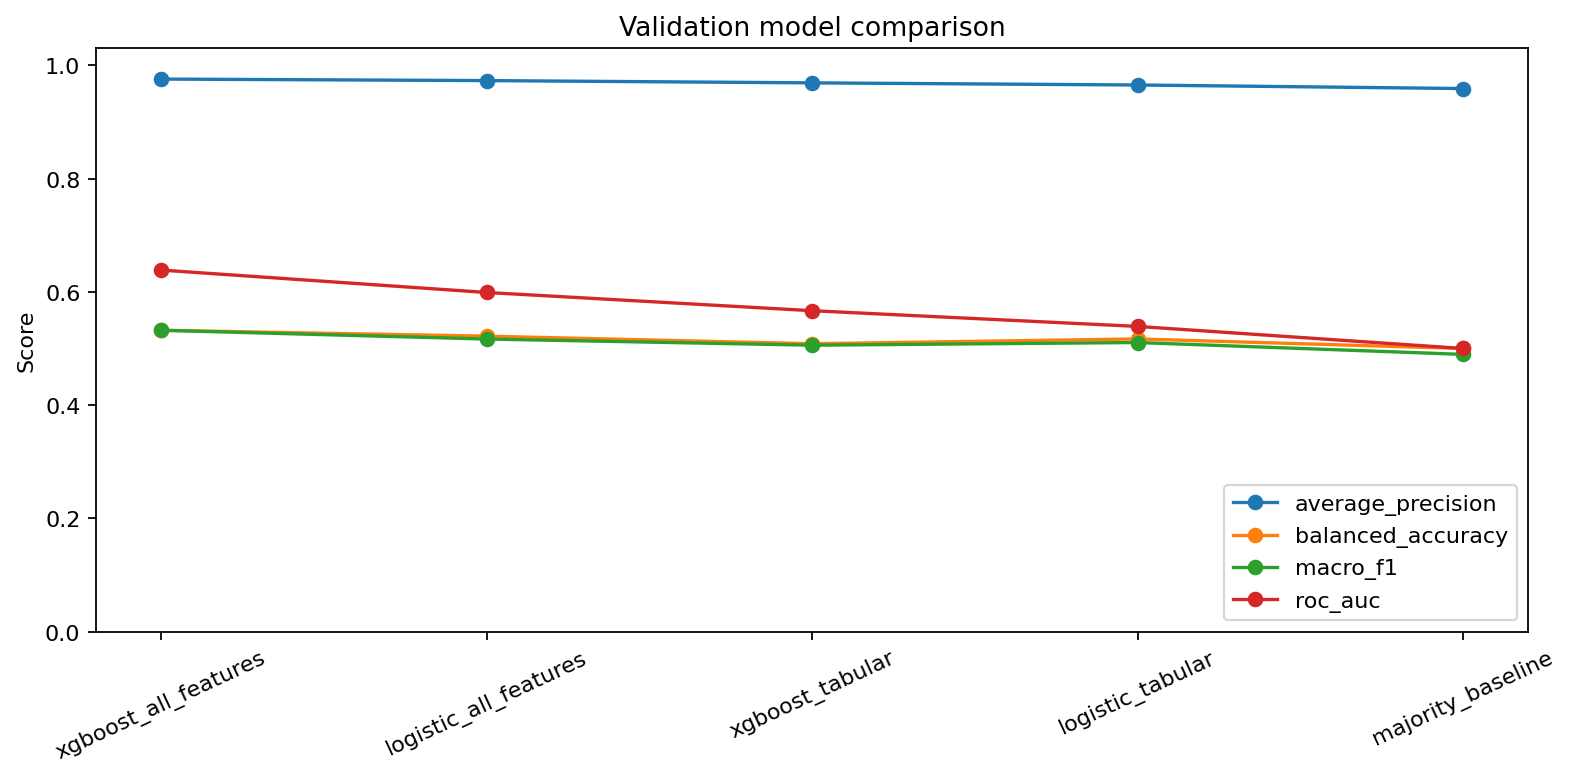
\includegraphics[width=\linewidth]{figures/modeling/model_comparison_validation.png}
    \caption{Validation metric comparison across model candidates.}
\end{figure}

\subsection{Assess Model}

The selected model is XGBoost with tabular features and code-diff embeddings. On the held-out test split it reaches ROC-AUC 0.628, PR-AUC 0.976, macro-F1 0.537, and balanced accuracy 0.534. The test confusion matrix is \([[4,36],[30,911]]\).

The high PR-AUC should be interpreted carefully. The positive class dominates the dataset, so even the majority baseline has PR-AUC 0.959. ROC-AUC, macro-F1, and balanced accuracy are more informative here. They show that the model has learned some ranking signal, but the separation between concerned and non-concerned pull requests remains weak.

The confusion matrix makes the limitation clear. The model correctly identifies most positive examples, but it detects only 4 of 40 negative examples in the test split. In other words, the model is much better at preserving recall for likely review concerns than at confidently recognizing pull requests without concern signals. This is acceptable as a baseline proving that the dataset contains signal, but it is not reliable enough for an automated decision system.

The likely reason is that review concern is not determined only by local diff text. Reviewers react to hidden project conventions, architectural fit, missing tests, API compatibility, maintainability, prior knowledge of the codebase, and the intent behind the change. A 1,000-token pooled diff embedding compresses much of this context and may miss long-range dependencies across files. Stronger performance would likely require a more powerful language-model setup: longer-context code-aware encoders, fine-tuning on review outcomes, structured discussion context, repository history, or an LLM-style model that can reason over the full pull request trace rather than only a capped diff representation.

\begin{figure}[htbp]
    \centering
    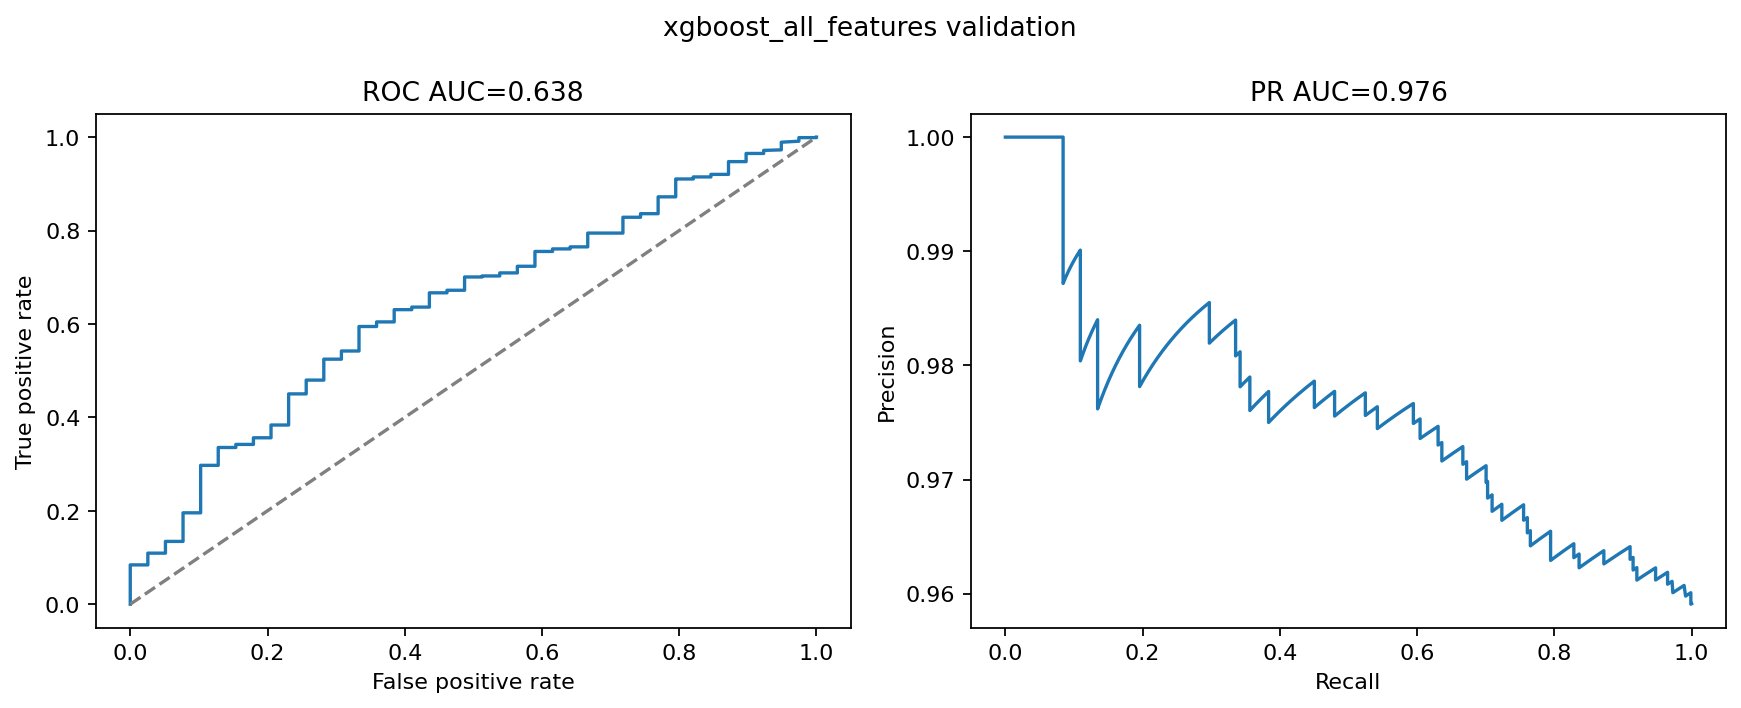
\includegraphics[width=\linewidth]{figures/modeling/selected_validation_curves.png}
    \caption{Selected model validation ROC and precision--recall curves.}
\end{figure}

\begin{figure}[htbp]
    \centering
    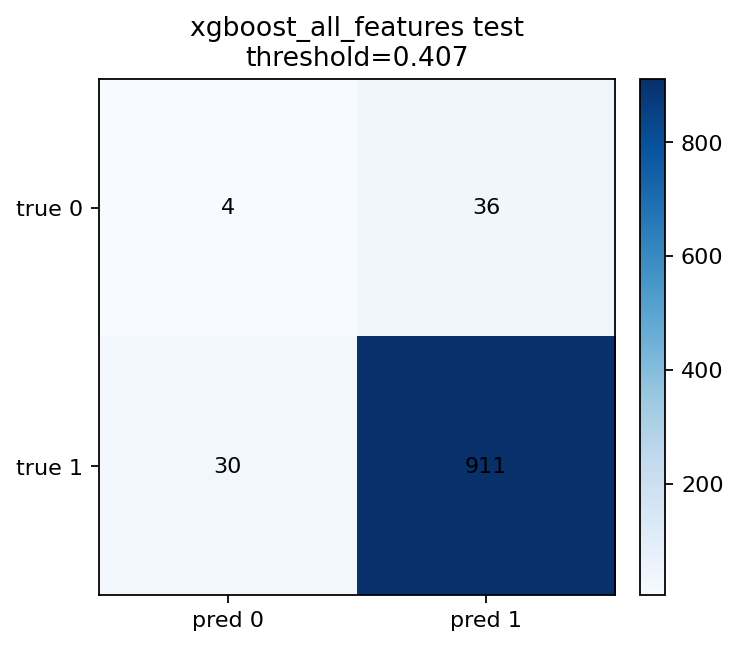
\includegraphics[width=.72\linewidth]{figures/modeling/selected_test_confusion.png}
    \caption{Selected model test confusion matrix.}
\end{figure}
